\documentclass[]{report}
\usepackage{etoolbox}
\usepackage{polski}
\usepackage[utf8]{inputenc}
\usepackage{geometry}
\usepackage{color,soul}
\usepackage{sidecap}
\usepackage{blindtext}
\usepackage{amsmath}
\usepackage{wrapfig}
\definecolor{codegray}{gray}{0.9}
\newcommand{\code}[1]{\colorbox{codegray}{\texttt{#1}}}
\usepackage{graphicx}
\usepackage{hyperref}
\newcommand{\link}[1]{{\color{blue}\href{#1}{#1}}}
\usepackage{xcolor}
\hypersetup{
	colorlinks,
	linkcolor={red!50!black},
	citecolor={blue!50!black},
	urlcolor={blue!80!black}
}
\graphicspath {{graphics/}}

\begin{document}
\newgeometry{tmargin=1.3cm, bmargin=1.3cm, lmargin=2cm, rmargin=2cm}
\title{Blastback \\
	\Large Raport z przebiegu projektu}
\maketitle



\stepcounter{chapter}
\chapter*{Aspekt sieciowy}
\section{Przyjęte założenia}
Aspekt sieciowy zrealizowaliśmy z pomocą sieciowego API \code{SpiderMonkey}, które jest dostarczone przez nasz silnik. Zapewnia ono podstawowe metody do łączenia się poprzez TCP/UDP, szablony wiadomości i podstawową klasę reagujących na nie Listenerów. Stan gry symulowany jest po stronie klienckiej, a serwer odpowiedzialny jest za wzajemną komunikację aplikacji klienckich poprzez nasłuchiwanie wiadomości i przekazywanie ich do reszty graczy.

\section{Symulacja po stronie klienta}
Po bliższym zapoznaniu się z technologią \code{jMonkeyEngine} oraz dostępnymi bibliotekami, doszliśmy do wniosku, że implementacja symulacji po stronie serwera oraz odpowiedniej interpretacji danych przez klienta pochłonęłaby zbyt wiele czasu, a bez odpowiednich mechanizmów predykcji i rekompensacji pingu, gracz czułby zbyt duże opóźnienia co w znaczny sposób wpłynęłoby na odczucia z rozgrywki. To skłoniło nas do implementacji symulacji po stronie klienta. Przyjęliśmy także założenia: opóźnienia sieci będą pomijalne oraz gracz nie będzie próbował oszukiwać.


\begin{itemize}
	\item \textbf{Gracz lokalny} \\
	Aplikacja kliencka wyróżnia obiekt lokalnego gracza i może bezpośrednio wpływać tylko na ten obiekt, głównie w wyniku działania użytkownika (sterowanie za pomocą klawiatury i myszki), a także algorytmów silnika fizycznego (\code{jBullet}) dostępnego w \code{jMonkeyEngine}. Gdy nawiązane jest połączenie z serwerem, klient wysyła z określoną częstotliwością informacje dotyczące obecnej pozycji oraz rotacji obiektu lokalnego gracza. W wyniku zdarzeń takich jak wystrzelenie pocisku, trafienie, śmierć lokalnego gracza, bezzwłocznie wysyłane są wiadomości informujące o tych zdarzeniach.
	\item \textbf{Symulacja - poruszanie} \\
	Aby gracz widział innych klientów podłączonych do danego serwera, wszystkie inne postaci są symulowane na podstawie wiadomości otrzymanych z serwera. Serwer zbiera aktualizacje stanów obecnie podłączonych graczy, tworzy z nich listę a następnie rozsyła ją do wszystkich klientów. Ze względu na to, że wiadomości dotyczące zmian pozycji gracza wysyłane są z częstotliwością znacznie mniejszą niż odświeżanie ekranu, pozycje symulowanych obiektów są interpolowane aby zapewnić ich płynny ruch.
	\item \textbf{Symulacja - pociski} \\
	Aby symulować pociski wystrzelone przez innych klientów, każdy klient wysyła wiadomość informującą o swoich wystrzale, a następnie ta wiadomość jest broadcastowana przez serwer do pozostałych klientów. W przypadku odebrania takiej wiadomości, aplikacja klienta tworzy obiekt symulowanego pocisku na podstawie informacji zawartych w wiadomości.
	\item \textbf{Symulacja - trafienia} \\
	Aby uniknąć duplikowania się wiadomości o trafieniach, jedynie pociski lokalne (wystrzelone przez lokalnego gracza) po skolidowaniu z symulowaną postacią wysyłają wiadomości do serwera. Symulowane pociski w wypadku kolizji jedynie znikają, nie wysyłając żadnych informacji.
	\item \textbf{Konsekwencje rozwiązania} \\
	Zaimplementowany przez nas sposób komunikacji jest skuteczny przy przyjętych przez nas założeniach, ale niestety bardzo szybko uwidaczniają się problemy, gdy któreś z tych założeń nie jest spełnione. W przypadku wystarczająco dużych opóźnień sieciowych, widoczne stają się różnice w symulacjach poszczególnych klientów, co powoduje problemy takie jak “trafienia znikąd” - gracz widzi utratę punktów życia, mimo tego że żaden pocisk go nie trafił. Nie ma też jakiegokolwiek mechanizmu broniącego przed oszustwami, w wyniku czego (np. przy pomocy \code{CheatEngine}) gracz może wpływać na aplikację tak aby uzyskać przewagę nad innymi użytkownikami.
\end{itemize}

\clearpage

\section{Rodzaje wiadomości}
W projekcie zaprojektowaliśmy własną klasę wiadomości \code{BaseBlastbackMessage} bazującą na dostarczonym szablonie, a następnie zaimpementowaliśmy 7 dziedziczących klas, odpowiedzialnych za przesyłanie konkretnych danych. Zarówno serwer jak i aplikacja kliencka dysponują Listenerami, które rozpoznają rodzaj przychodzącej wiadomości i w odpowiedni sposób ją obsługują. 
Każda z wiadomości posiada odpowiadającą jej klasę z danymi, które serializowane są w momencie utworzenia wiadomości i deserializowane przy obsługiwaniu po dotarciu do serwera lub innego klienta. 
Zaimplementowanie wielu różnych rodzajów wiadomości dało nam możliwość sprawnego komunikowania o zdarzeniu danego typu, które wywołują wysłanie odpowiedniego komunikatu, tym samym zmniejszając ilość niezbędnych danych w \code{PlayerStateInfosMessage}, które rozsyłane są nieustannie by zapewnić informacje o symulacji innym klientów.

\begin{align*}
 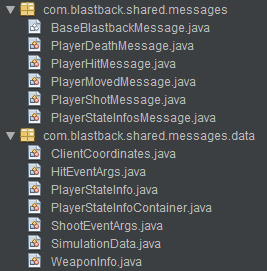
\includegraphics[scale=0.7]{messages}
\end{align*}


\section{Serializacja}
W trakcie realizacji projektu uznaliśmy że prawidłowy przesył danych jest niezbędny do prawidłowego działania programu, stąd nasza decyzja na serializację danych przesyłanych poprzez wiadomości do formatu json z pomocą biblioteki \code{gson}.
Problemy biblioteki \code{gson}, takich jak serializacja klas generycznych, spowodowały, że zdecydowaliśmy się na implementację klas przechowujących dane, które następnie będą wysłane.
Json zapewnił danym elastyczności niezbędnej w stale rozwijającej się aplikacji, pozwalając dowolnie kształtować klasy przetrzymujące dane wiadomości, bez konieczności tworzenia na szybko własnych, zawodnych mechanizmów deserializacji. 



\stepcounter{chapter}
\chapter*{Grafika i dźwięk}
Grafika składa się z modeli które zostały stworzone w programie \code{Blender}.
Modele utworzone w tym programie zostały zaimportowane do projektu.
Następnie modele zostały odpowiednio podczepione pod scenę, w celu ich renderowania.
Model postaci jest ładowany przy dołączeniu do gry, a następnie jest przemieszczany po mapie przy pomocy pozycji obiektu w przestrzeni.
Fizyka całego rozwiązania opiera się na fizyce silnika \code{jMonkeyEngine}.
Każdy obiekt posiada informacje o ich kształcie kolizyjnym, który jest wykorzystywany do detekcji kolizji.
W przypadku wykrycia kolizji wykonywane są odpowiednie akcje.
Muzyka która gra w tle jest realizowana przy pomocy silnika \code{jMonkeyEngine} który odtwarza wybrany utwór w pętli na całej mapie dla każdego klienta indywidualnie.
Dźwięk strzału broni wywołujemy przy pomocy eventów, które umożliwiają na odtworzenie odpowiedniego dźwięku dla wybranej broni przy pomocy argumentów przesyłanych razem z eventem.


\stepcounter{chapter}
\chapter*{Interfejs użytkownika}
\section{NiftyGUI}
Interfejs graficzny w naszej aplikacji jest renderowany przy użyciu \code{NiftyGUI}. Jest to oprogramowanie typu open source, dostępne pod linkiem \link{https://github.com/nifty-gui/nifty-gui}. Wykorzystuje bibliotekę graficzną \code{OpenGL}. Rozwijając aplikację w \code{jMonkeyEngine} mieliśmy do wyboru jeszcze 3 inne rozwiązania: \code{Swing}, \code{Lemur}, \code{tonegodGUI} oraz powszechnie stosowany. Niestety dobrze nam znane pierwsze rozwiązanie nie jest dobrze zintegrowane z silnikiem, a drugie okazało się być nierozwijane już od 3 lat: \link{https://github.com/meltzow/tonegodgui}.Wybraliśmy \code{NiftyGUI} zamiast \code{Lemur}, ponieważ możliwość definiowanią układu kontrolek oraz ich styli w xml wydawała nam się najlepszym rozwiązaniem.


\section{Układ elementów na ekranie}
\code{NiftyGUI} jest oprogramowaniem, w którym do projektowania układu elementów można wykorzystać język znaczników xml. Alternatywnie można robić to też przy użyciu kodu javowego. Uznaliśmy jednak, że xml będzie bardziej przejrzystym rozwiązazniem. Definicje układów wszystkich ekranów wyświetlanych użytkownikowi znajdują się w \code{assets/Interface/Screens/screens.xml}.

\section{Stylowanie kontrolek}
Aby odpowiednio wystylować wygląd kontrolek pod nasze potrzeby, należało przeciążać ich domyślne style. Nasze definicje styli zostały również zapisane w pliku xml i znajdują się w \code{assets/Interface/Styles/styles.xml}. Powyżej - wygląd głownego menu gry z przeciążonymi definicjami stylów, poniżej - ich domyślne odpowiedniki.
\begin{gather*}
	\includegraphics*[scale=0.32]{gui_styled} \\
	\includegraphics*[scale=0.32]{gui_not_styled} 
\end{gather*}


\stepcounter{chapter}
\chapter*{Podsumowanie}
\section{Propozycje rozwoju}
\section{Wnioski po pracy z silnikiem}




\end{document}
